\section{Introduction} \label{sec:intro}


The Vera C. Rubin Observatory is located at Cerro Pachón in the Atacama Desert in Chile. It was chosen after considering different sites worldwide according to their meteorological conditions. It will operate the 8.4-meter Simonyi Research Telescope, which will be able to scan the entire southern sky in approximately three nights and is expected to start operations in 2024. This observatory also has the giant camera ever built, the LSST Camera, which has a 3.2 gigapixel resolution for the entire focal plane, with a diameter of 64 cm to cover 9.6 deg$^2$ FoV and a plate scale of 0.2 '' pixel$^-1$ \citep{2009arXiv0912.0201L}.

\vspace{3mm}

This observatory is named in honor of the astronomer Vera Rubin  \citep{NSF_2020}, who in 1970 pioneered the measurement of the rotation curves of disk galaxies \citep{rubin2011interesting}, in which she realized that for the stars in galaxies to rotate at the rate they do, there must be more mass than we observe for the galaxies not to break apart. This mass is what we now call dark matter, which is one of the scientific goals of this observatory. 

\vspace{3mm}

Vera Rubin received several awards, including the National Medal of Science, and even a ridge on Mars is named after her \citep{koren_2020}. In addition, she worked hard for the recognition of the work of women in science and her students \citep{rubin2011interesting}. 


\subsection{LSST Scientific goals}

The LSST has four main scientific objectives \citep{2009arXiv0912.0201L, ivezic2019lsst}:

\begin{itemize}
    \item Taking an Inventory of the Solar System: The minor bodies of the solar system, such as TNOs, asteroids, and comets, are crucial to understanding planetary formation and evolution since their orbital elements and sizes preserve this history. On the other hand, the interaction of objects in the Main Asteroid Belt, which lies between Mars and Jupiter, could launch some of these objects into Earth's orbit, so their study will help to make a connection between NEOs coming from the Main Belt. 
    
    \item Mapping the Milky Way: It concerns the study of the formation and evolution of our galaxy by observing its stars' structure, dynamics, and chemical composition. In addition, this science objective will characterize the stars in the solar neighborhood (300 pc).
    
    \item Exploring the Transient Optical Sky: This time domain science observes transient and variable phenomena such as supernovae, variable stars, and AGN. The goal is to detect transient and distant objects. This requires several properties: covering a large part of the sky to increase the probability of seeing these events, good quality images to observe the differences between images, good sampling time to detect the different types of variable stars, accurate color information for classification, long-term persistent observations to follow up the event, reduction, classification and rapid publication to the community to allow the study of these objects in other fields, such as spectroscopy. 
    
    \item Probing Dark Energy and Dark Matter: Dark energy affects the universe's expansion as the accumulation of mass, so the observations must depend on the redshift to study it. For this purpose, they will study weak gravitational lensing, large-scale structures such as galaxy clusters, BAO (Baryonic AcoAcousticcillation), and Supernova systems, among others. For the study of dark matter, there are several mechanisms to explore it, such as weak and strong lensing of galaxy mass distributions.. 
\end{itemize}

\subsection{What kind of CCD does the LSST Camera have?}
The LSSTCam is composed of \textit{thick fully depleted} and back-illuminated CCDs\citep{2009arXiv0912.0201L}. This type of CCD is characterized by a good response in the near-infrared regions \citep{lage2017measurements}, which allows observation of distant objects reddened by the universe's expansion. However, being thick, they present some effects due to the long path that the generated electrons must travel to the charge storage well. 

\vspace{3mm}

The LSSTCam is highly segmented, which enables it to be read out completely in 2 s and reduces the readout noise produced by high readout speeds \citep{2009arXiv0912.0201L}. It comprises a mosaic of 205 CCDs organized by 21 science modules, each containing nine CCDs and four specialized corner modules for telescope guidance and alignment by active optics \citep{snyder2020laboratory}. This mosaic has CCDs from two vendors: Imaging Technology Laboratories (ITL) and Teledyne e2v (E2V), and each is divided into 16 segments. Figure \ref{fig:FP_LSSTCam} shows in yellow the vendor's E2V detectors, in greenish blue the ITL detectors, which are the science CCDs, and in purple the guidance CCDs. 

\vspace{3mm}

According to \cite{walter2015brighter} for the LSST science objective in weak lensing, where the aim is to measure how this modifies the shape of galaxies by observing a wide field, it is crucial to quantify the brighter-fatter (BF, hereafter) effect since exact measurements of the PSF of galaxies are required. The BF effect leads to the deformation of the PSF, being more critical in bright objects and progressively decreasing in fainter objects \citep{lage2017measurements}. On the other hand, \cite{walter2015brighter} mentions that another effect suffered by the sensors is the edge effect, where electrons near the edge of the sensor feel a force that pushes them inward, which mainly affects astrometry.



\begin{figure}[!htb]
    \centering
    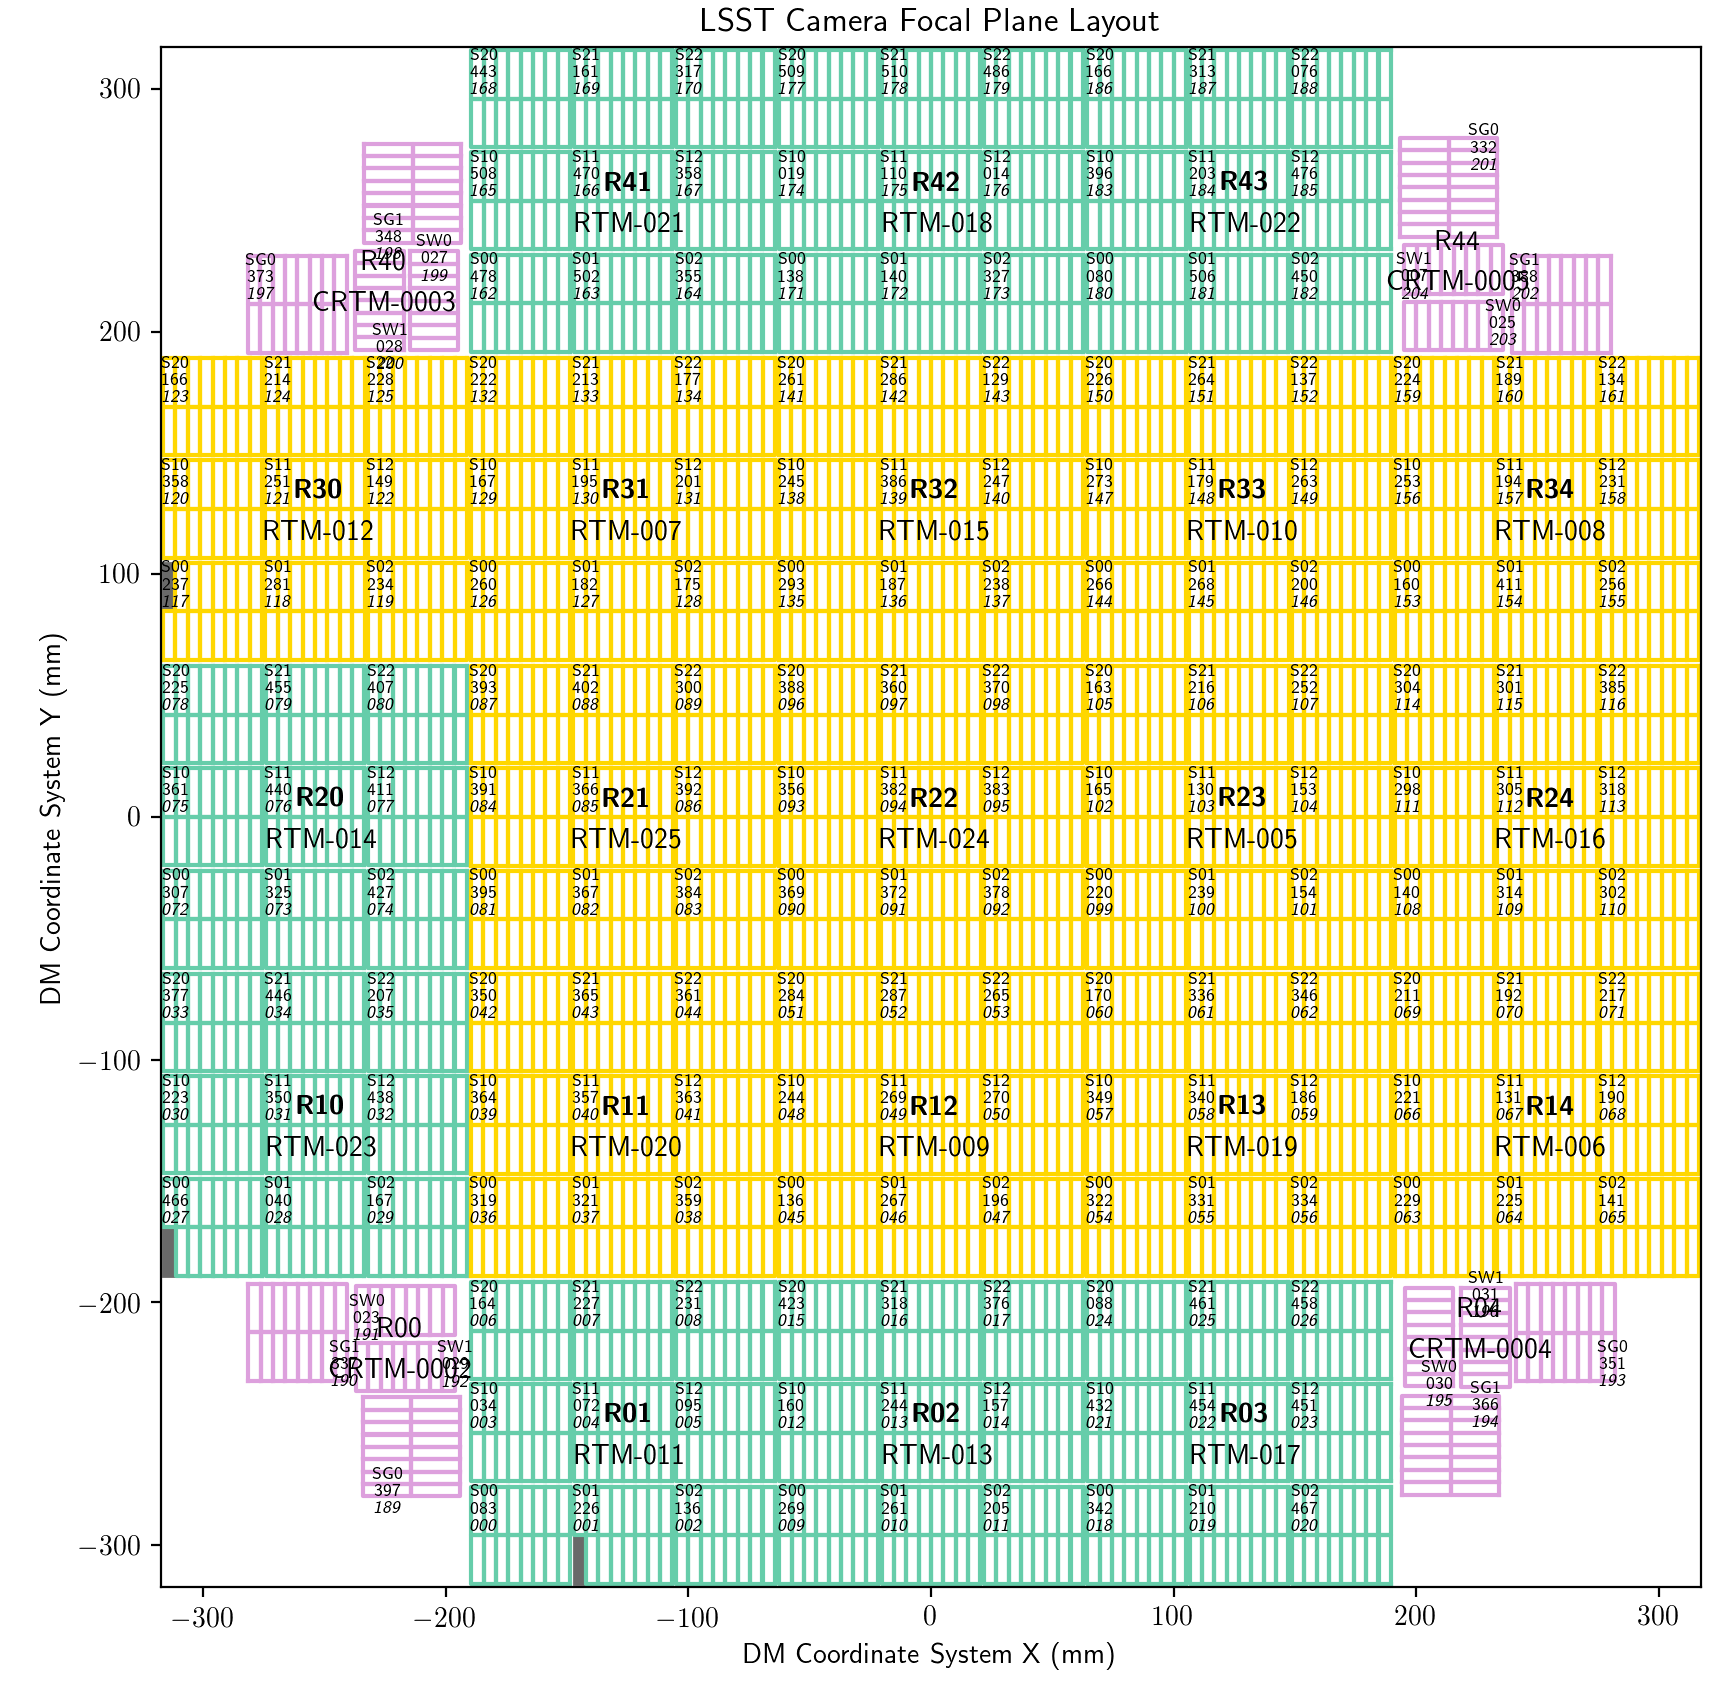
\includegraphics[width=\textwidth]{Figures/FP_layout_DM.png}
    \caption{The focal plane of the LSST camera. The vendor's CCDs' location is blue for ITL and yellow for E2V. Each CCD (a small square) is composed of 16 segments, each with its amplifier, and 189 CCDs are responsible for taking the science data. The CCDs at the corners are for focusing and synchronization with the Earth's rotation (see \href{https://www6.slac.stanford.edu/news/2020-09-08-sensors-world-largest-digital-camera-snap-first-3200-megapixel-images-slac.aspx}{LSST-SLACLab})}
    \label{fig:FP_LSSTCam}
\end{figure}

\subsection{What is Photon Transfer Curve (PTC)?}

The Photon Transfer Curve (PTC) allows the characterization of the fundamental parameters of the CCD, mainly the determination of the relationship between the electrons recorded by each pixel and their conversion to analog-to-digital counts (ADU), i.e., the gain; it also measures the nonlinearity of the camera and its Full Well Capacity (FWC). The first parameter is essential because other vital parameters, such as read noise, quantum efficiency, dark current, among others, depend on it \citep{downing2006ccd}.

Figure \ref{fig:PTC} shows the PTC of segment C06 of sensor 22 of the LSSTCam, where it is evident that at low fluxes, the variance is low and increases with the flux but not linearly until the saturation point or FWC, which for this detector is $83000$ ADU. After this point, the variance begins to decrease, indicating that the flux stored in each pixel of this amplifier begins to homogenize. The nonlinear behavior of this curve is exhibited by \textit{thick fully-depleted CCDs}, according to \cite{downing2006ccd} charge storage in a pixel is the main reason, since the expected relationship between the variance and the mean number of counts in a pixel is modified in flat images \citep{walter2015brighter}. The effective area of the pixel changes with the amount of charge, decreasing the more significant the charge accumulated in the pixel. Consequently, very bright sources are mainly affected by this so-called BF effect. If the pixels of the CCD segment were independent, they could be described by Poisson statistics, and the PTC would follow the green line in the figure.

\begin{figure}[!htb]
    \centering
    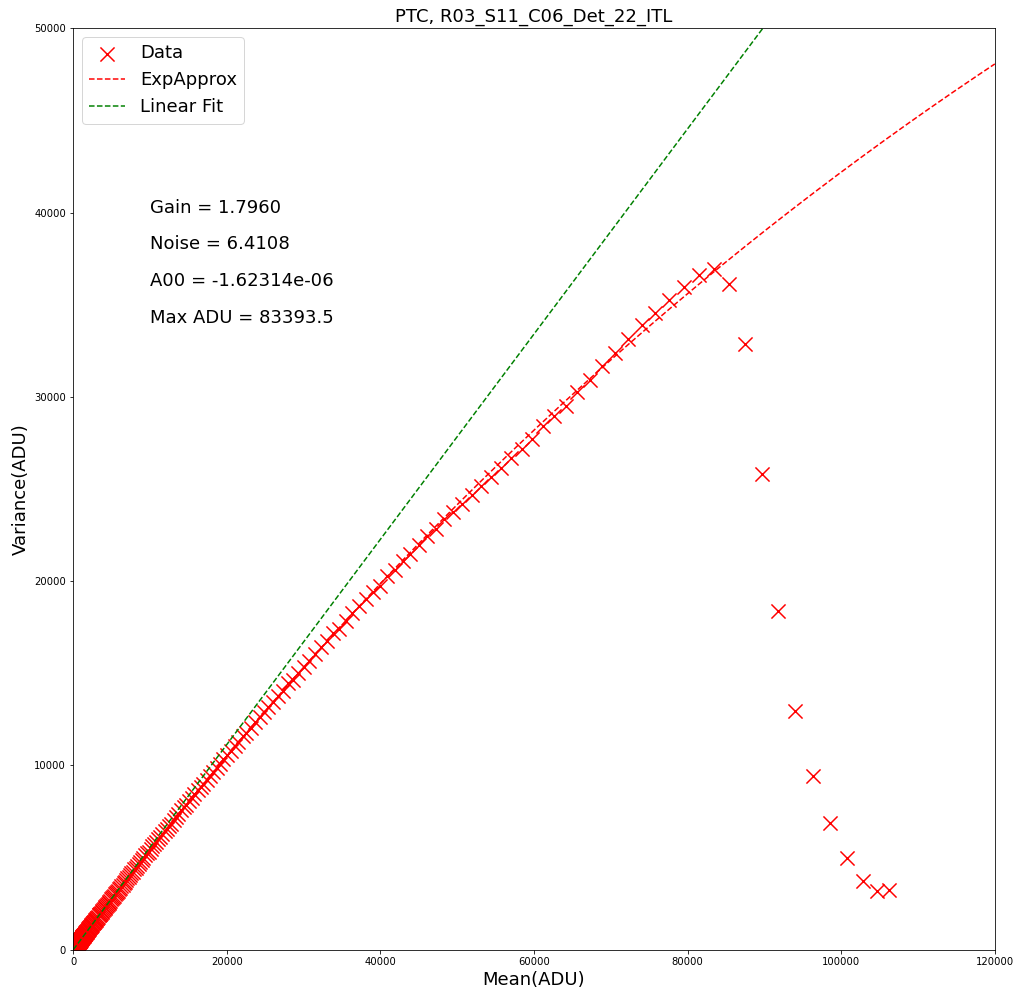
\includegraphics[width=0.7\textwidth]{Figures/PTC_R03_S11_C06_Det22.png}
    \caption{PTC for detector 22 was found in raft 03, sensor 11, and amplifier C06; its vendor is ITL. In red crosses, the data are shown, the red line uses the EXPAPPROXIMATION fit, and the green line is a linear fit. This curve was constructed with the results obtained via \textit{DM stack}.}
    \label{fig:PTC}
\end{figure}

\subsubsection{Brigther father effect}

As mentioned above, the charge stored in a pixel modifies the effective area of the pixel, decreasing the probability that this pixel will continue to store the charge. Consequently, the electrons that should have been kept in this pixel are deflected horizontally, causing more elliptical images. Thus, a process initially described by a Poisson statistic, and the charge stored in each pixel was independent of the other, breaks down by modifying the relationship between the variance and the mean number of counts per pixel \citep{walter2015brighter}. This effect changes the PSF, so it is a potential problem in surveys interested in the variation of the brightness and shape of objects \citep{coulton2018exploring}


\vspace{6mm}


This work was developed during the RECA (Red de Estudiantes Colombiana de Astronomía) internship program 2022\footnote{RECA internship program is a training program in scientific research in Astronomy, Astrophysics, and Cosmology directed to students of Colombian institutions. The program website \href{https://recastronomia.github.io/internship/}{https://recastronomia.github.io/internship/}}. The program was carried out over three months, in which we also developed other activities such as remote astronomical observations with the Teide Observatory\footnote{\href{https://www.iac.es/es/observatorios-de-canarias/observatorio-del-teide}{https://www.iac.es/es/observatorios-de-canarias/observatorio-del-teide}}.


In this report, we present the data used in the section \ref{sec:data}. The section \ref{sec:methods} describes the methodology used. In the section \ref{sec:results}, we present the results and analysis. Finally, the conclusion in section\ref{sec:conclusions}.